\newpage
\section{Đề thi Giải tích}

\begin{tcolorbox}[title=\textbf{Bài toán B.1 + A.1.},breakable]
    Cho $(a_n)$ là dãy số thực được xác định bởi các điều kiện $$a_1 = 1,\quad a_{n+1} = a_n + \dfrac{(-1)^n}{n!} \,\forall n \geq 1.$$
    \begin{enumerate}
        \item[(a)] {Tìm tất cả các số nguyên dương $n$ sao cho $a_n \geq \dfrac{1}{2}$.}
        \item[(b)] {Chứng minh rằng dãy số $(a_n)$ hội tụ.} 
        \item[(c)] Giới hạn của dãy số $(a_n)$ là một số hữu tỷ hay vô tỷ? Vì sao? 
    \end{enumerate}
\end{tcolorbox}

\textbf{Lời giải. }

\begin{enumerate}
    \item[(a)] {Bằng tính toán, ta có $a_1 = 1,\,a_2 = 0,\,a_3 = \dfrac{1}{2},\,a_4 = \dfrac{1}{3},\,a_5 = \dfrac{3}{8}$. Ta sẽ chứng minh rằng $a_n < \dfrac{1}{2}$ với mọi $n > 3$. 
    
    Thật vậy, mệnh đề cần chứng minh đúng với $n = 4$ và $n = 5$. Giả sử mệnh đề đúng đến $n = 2k$ và $n = 2k + 1$ (trong đó $k \in \mathbb{Z^+}$), tức đã có $a_{2k} < \dfrac{1}{2}$ và $a_{2k+1} < \dfrac{1}{2}$. Ta có $$a_{2k + 2} = a_{2k+1} - \dfrac{1}{(2k + 1)!} < \dfrac{1}{2}$$ và $$a_{2k+3} = a_{2k+2} + \dfrac{1}{(2k+2)!} = a_{2k+1} - \dfrac{1}{(2k+1)!}+ \dfrac{1}{(2k+2)!} = a_{2k+1} - \dfrac{2k}{(2k+2)!} < \dfrac{1}{2}.$$
    
    Như vậy theo nguyên lý quy nạp toán học, $a_n < \dfrac{1}{2}$ với mọi $n > 3$. Do đó tất cả các số nguyên dương $n$ thỏa mãn $a_n \geq \dfrac{1}{2}$ là 1 và 3.} 
    \item[(b)] {Với mọi $n\geq 2$ ta có $$a_n = a_{n-1} + \dfrac{(-1)^{n-1}}{(n-1)!} = a_{n-2} + \dfrac{(-1)^{n-1}}{(n-1)!} + \dfrac{(-1)^{n-2}}{(n-2)!} = \cdots = a_1 + \sum\limits_{i = 1}^{n-1}\dfrac{(-1)^{i}}{i!} = 1 + \sum\limits_{i = 1}^{n-1}\dfrac{(-1)^{i}}{i!}.$$
    
    Xét hàm số $f(x) = {\rm e}^{-x}$. Ta thấy $$f^{(n)}(x) = \begin{cases}
        -{\rm e}^{-x},\quad &\text{nếu $n$ lẻ} \\
        {\rm e}^{-x},\quad &\text{nếu $n$ chẵn}  
    \end{cases},$$ trong đó $f^{(n)}(x)$ là đạo hàm cấp $n$ của hàm số $f$. Theo khai triển Maclaurin, ta có $$f(x) = 1 + \dfrac{-1}{1!}x + \dfrac{1}{2!}x^2 + \cdots + \dfrac{(-1)^{n-1}}{(n-1)^n}x^{n-1} + \dfrac{(-1)^n \cdot {\rm e}^{-c}}{n!}x^n,$$
    trong đó $c$ là số thực nào đó nằm giữa 0 và $x$.
    
    Từ đây suy ra $$\dfrac{1}{{\rm e}} = f(1)  = 1 + \dfrac{-1}{1!} + \dfrac{1}{2!} + \cdots + \dfrac{(-1)^{n-1}}{(n-1)^n} + \dfrac{(-1)^n \cdot {\rm e}^{-c}}{n!}= a_n + \dfrac{(-1)^n \cdot {\rm e}^{-c}}{n!},$$ với $c$ là số thực nào đó thỏa mãn $0 < c < 1$, với mọi $n \geq 2$.
    
    Do đó với mọi $n \geq 2$ thì $$\left|a_n - \dfrac{1}{{\rm e}}\right| = \dfrac{{\rm e}^{-c}}{n!}, $$ với $c$ là số thực nào đó thỏa mãn $0 < c < 1$.
    
    Trong đẳng thức trên, cho $n \to +\infty$, để ý rằng $\dfrac{{\rm e}^{-c}}{n!} \to 0$, ta thu được $\lim\limits_{n\to +\infty}a_n = \dfrac{1}{{\rm e}}$. Như vậy dãy số $(a_n)$ hội tụ.} 
    \item[(c)] {Theo câu (b), ta có $\lim\limits_{n\to +\infty}a_n = \dfrac{1}{{\rm e}}$ là một số vô tỷ.} 
\end{enumerate}

\textbf{Nhận xét. }Đây là một bài toán giới hạn dãy số liên quan giới hạn của chuỗi số. Câu (a) là một câu cơ bản, đòi hỏi việc tính toán một số giá trị đầu của dãy số và kỹ năng chứng minh quy nạp. Câu (b) có thể tách dãy số đã cho làm hai dãy con chẵn và lẻ, từ đó sử dụng định nghĩa để chứng minh; cách giải đề xuất ở đây có phần gọn hơn, nhưng đòi hỏi phải nhận xét được dãy số đã cho liên quan đến khai triển Maclaurin của hàm $f(x) = {\rm e}^{-x}$. Tuy nhiên cách giải được đề xuất ở đây lại hiệu quả trong việc chỉ ra chính xác giới hạn của dãy $(a_n)$ là $\dfrac{1}{{\rm e}}$.

\begin{tcolorbox}[title=\textbf{Bài toán B.2 + A.2.},breakable]
    Cho $f:\,\mathbb{R} \to \mathbb{R}$ là hàm số được xác định bởi công thức $$f(x) = \begin{cases}
        ax^2+b,\quad &\text{nếu $x \leq 0$} \\
        {\rm e}^x + cx,\quad &\text{nếu $x > 0$}  
    \end{cases},$$trong đó $a,\,b,\,c$ là các tham số thực.
    \begin{enumerate}
        \item[(a)] {Xác định $a,\,b,\,c$ sao cho hàm $f$ liên tục trên $\mathbb{R}$.}
        \item[(b)] {Xác định $a,\,b,\,c$ sao cho hàm $f$ khả vi trên $\mathbb{R}$.} 
        \item[(c)] {Xác định $a,\,b,\,c$ sao cho hàm $f$ khả vi cấp hai trên $\mathbb{R}$.} 
    \end{enumerate}
\end{tcolorbox}

\textbf{Lời giải. }

\begin{enumerate}
    \item[(a)] {Với $x \leq 0$ thì $f(x) = ax^2 + b$, còn với $x > 0$ thì $f(x) = {\rm e}^x + cx$ nên $f$ liên tục tại mọi điểm khác 0. Do đó để $f$ liên tục trên $\mathbb{R}$ thì $f$ cần phải liên tục tại $0$.
        
    Ta có $$\lim\limits_{x \to 0^-}f(x) = \lim\limits_{x \to 0^-} (ax^2 + b) = b,\quad \lim\limits_{x \to 0^+}f(x) = \lim\limits_{x \to 0^+}({\rm e}^x + cx) = 1 = f(0).$$ 
    
    Để $f$ liên tục tại $0$ thì $\lim\limits_{x \to 0^-}f(x) = \lim\limits_{x \to 0^+}f(x) = f(0)$ hay $b = 1$. Như vậy khi $b = 1$ và $a,\,c$ tùy ý thì $f$ liên tục trên $\mathbb{R}$.}
    \item[(b)] {Nhận xét rằng $f$ khả vi tại mọi điểm khác 0. Do đó để $f$ khả vi trên $\mathbb{R}$ thì $f$ cần phải khả vi tại 0. Điều này tương đương với $$\begin{cases}
        \text{$f$ liên tục tại 0} \\
        \text{$\lim\limits_{x \to 0}\dfrac{f(x) - f(0)}{x}$ tồn tại}
    \end{cases}.$$
    
    Theo câu $(a)$, để $f$ liên tục tại 0 thì $b = 1$. 
    
    Ta có $$\lim\limits_{x \to 0^-}\dfrac{f(x) - f(0)}{x} = \lim\limits_{x \to 0^-}\dfrac{ax^2 + b - b}{x} = \lim\limits_{x \to 0^-}ax = 0$$ và $$\lim\limits_{x \to 0^+}\dfrac{f(x) - f(0)}{x} = \lim\limits_{x \to 0^+}\dfrac{{\rm e}^x + cx - 1}{x} = c + 1,$$ để ý rằng $\lim\limits_{x \to 0^+} \dfrac{{\rm e}^x-1}{x} = \lim\limits_{x \to 0^+} \dfrac{{\rm e}^x}{1} = 1$ theo quy tắc l'Hospital.
    
    Do đó để $\lim\limits_{x \to 0}\dfrac{f(x) - f(0)}{x}$ tồn tại thì $\lim\limits_{x \to 0^-}\dfrac{f(x) - f(0)}{x} = \lim\limits_{x \to 0^+}\dfrac{f(x) - f(0)}{x}$ hay $c = -1$. Như vậy, khi $b = 1,\,c = -1$ và $a$ tùy ý thì $f$ khả vi trên $\mathbb{R}$.}
    \item[(c)] {Để $f$ khả vi cấp hai trên $\mathbb{R}$ thì trước hết $f$ phải khả vi cấp một trên $\mathbb{R}$. Theo câu (b), để $f$ khả vi cấp một trên $\mathbb{R}$ thì $b = 1,\,c = -1$ và khi đó $$f'(x) = \begin{cases}
        2ax,\quad &\text{nếu $x \leq 0$} \\
        {\rm e}^x - 1,\quad &\text{nếu $x > 0$} \\
        \lim\limits_{x \to 0}\dfrac{f(x) - f(0)}{x} = 0,\quad &\text{nếu $x = 0$} 
    \end{cases}$$
        
    Nhận xét rằng $f$ khả vi cấp hai tại mọi điểm khác 0. Do đó để $f$ khả vi cấp hai trên $\mathbb{R}$ thì $f$ cần phải khả vi cấp hai tại 0. Điều này tương đương với $$\begin{cases}
        \text{$f'$ liên tục tại 0} \\
        \text{$\lim\limits_{x \to 0}\dfrac{f'(x) - f'(0)}{x}$ tồn tại}
    \end{cases}.$$
    
    Ta có $$\lim\limits_{x \to 0^-}f'(x) = \lim\limits_{x \to 0^-} (2ax) = 0,\quad \lim\limits_{x \to 0^+}f'(x) = \lim\limits_{x \to 0^+} ({\rm e}^x -1) = 0 = f'(0).$$
    
    Vì $\lim\limits_{x \to 0^-}f'(x) = \lim\limits_{x \to 0^+}f'(x) = f'(0)$ nên $f'$ liên tục tại 0.
    
    Ta lại có $$\lim\limits_{x \to 0^-}\dfrac{f'(x)-f'(0)}{x} = \lim\limits_{x \to 0^-}\dfrac{2ax}{x} = 2a$$ và $$\lim\limits_{x \to 0^+}\dfrac{f'(x)-f'(0)}{x} = \lim\limits_{x \to 0^+}\dfrac{{\rm e}^x - 1}{x} = 1.$$
    
    Do đó để $\lim\limits_{x \to 0}\dfrac{f'(x) - f'(0)}{x}$ tồn tại thì $\lim\limits_{x \to 0^-}\dfrac{f'(x) - f'(0)}{x} = \lim\limits_{x \to 0^+}\dfrac{f'(x) - f'(0)}{x}$ hay $a = \dfrac{1}{2}$. Như vậy, khi $a = \dfrac{1}{2},\,b = 1,\,c = -1$ thì $f$ khả vi cấp hai trên $\mathbb{R}$.}
\end{enumerate}

\textbf{Nhận xét. }Đây là một bài toán cơ bản về tính liên tục và khả vi của hàm số. Để giải quyết bài toán này đòi hỏi phải nắm vững tính chất về tính liên tục và tính khả vi.

Để hàm số $f$ liên tục tại điểm $x = x_0$ thì $f$ phải thỏa mãn đồng thời ba điều kiện 
\begin{enumerate}
    \item[(i)] {$f$ xác định tại $x_0$;}
    \item[(ii)] {$\lim\limits_{x\to x_0}f(x)$ tồn tại;}
    \item[(iii)] {$\lim\limits_{x\to x_0}f(x) = f(x_0)$.}
\end{enumerate}

Còn để hàm số $f$ khả vi tại điểm $x = x_0$ thì $f$ phải thỏa mãn đồng thời hai điều kiện 
\begin{enumerate}
    \item[(i)] {$f$ liên tục tại điểm $x = x_0$;}
    \item[(ii)] {$\lim\limits_{x\to x_0}\dfrac{f(x) - f(x_0)}{x - x_0}$ tồn tại.}
\end{enumerate}
khi đó $\lim\limits_{x\to x_0}\dfrac{f(x) - f(x_0)}{x - x_0}$ là đạo hàm của hàm số $f$ tại điểm $x = x_0$ hay $f'(x_0)$.

\begin{tcolorbox}[title=\textbf{Bài toán B.3 + A.3.},breakable]
    Hình vẽ bên thể hiện một phần đường thẳng $(d)$ có phương trình $$y = 2x - 1$$ và một phần parabol $(P)$ có phương trình $$y = 3x^2$$ trong mặt phẳng tọa độ $Oxy$.
    \begin{center}
        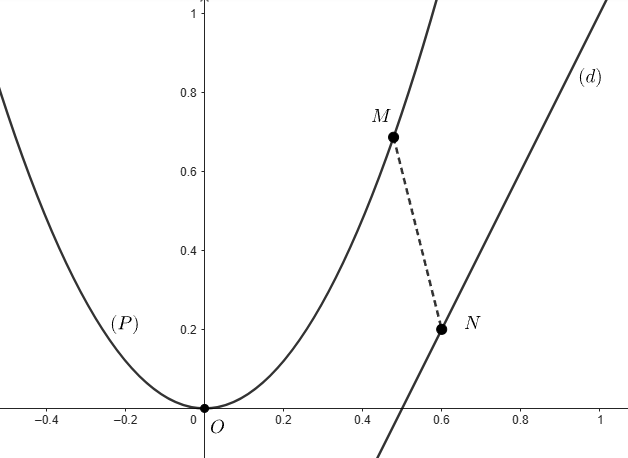
\includegraphics[width=0.5\textwidth]{Figures/04.png}
    \end{center}
    \begin{enumerate}
        \item[(a)] {Đường thẳng $(d)$ và parabol $(P)$ có cắt nhau không? Vì sao?}
        \item[(b)] {Cho các điểm $M \in (P)$ và $N\in (d)$. Tìm giá trị nhỏ nhất của khoảng cách $MN$.} 
    \end{enumerate}
\end{tcolorbox}

\textbf{Lời giải. }

\begin{enumerate}
    \item[(a)] {Xét phương trình hoành độ giao điểm $$3x^2 = 2x - 1 \iff 3x^2 - 2x + 1 = 0.$$
    
    Phương trình trên là phương trình bậc hai có $\Delta = (-2)^2 - 4\cdot 3 \cdot 1 = -8 < 0$ nên không có nghiệm thực. Như vậy $(d)$ và $(P)$ không cắt nhau.}
    \item[(b)] {Gọi $m,\,n$ lần lượt là hoành độ của $M,\,N$. Vì $M\in (P)$ và $N \in (d)$ nên ta có $M\left(m;\,3m^2\right)$ và $N\left(n;\,2n-1\right)$. Khi đó $$MN = \sqrt{(m-n)^2 + (3m^2 - 2n + 1)^2}.$$
    
    Xét hàm số (theo biến $n$) $$f(n) = (m-n)^2 + (3m^2 - 2n + 1)^2 = 5n^2 - (12m^2+2m+4)n + 9m^4 + 7m^2 + 1.$$
    
    Vì $f$ là hàm số bậc hai theo biến $n$ nên $f$ đạt cực tiểu tại $n = \dfrac{6m^2+m+2}{5}$, khi đó $$f\left(\dfrac{6m^2+m+2}{5}\right) = \dfrac{9}{5}m^4 - \dfrac{12}{5}m^3 + 2m^2 - \dfrac{4}{5}m + \dfrac{1}{5}.$$
    
    Nhận xét rằng $\dfrac{9}{5}m^4 - \dfrac{12}{5}m^3 + 2m^2 - \dfrac{4}{5}m + \dfrac{1}{5} = \left(m - \dfrac{1}{3}\right)^2\left(\dfrac{9}{5}m^2 - \dfrac{6}{5}m + 1\right) + \dfrac{4}{45} = \left(m - \dfrac{1}{3}\right)^2\left(\dfrac{1}{5}(3m - 1)^2 + \dfrac{4}{5}\right) + \dfrac{4}{45} \geq \dfrac{4}{45}$ với mọi $m$. Suy ra $MN^2$ đạt giá trị nhỏ nhất bằng $\dfrac{4}{45}$ khi $m = \dfrac{1}{3}$ và $n = \dfrac{6m^2+m+2}{5} = \dfrac{3}{5}$. Như vậy $MN$ đạt giá trị nhỏ nhất bằng $\dfrac{2\sqrt{5}}{15}$ khi $M\left(\dfrac{1}{3};\,\dfrac{1}{3}\right)$ và $N\left(\dfrac{3}{5};\,\dfrac{1}{5}\right)$.}
\end{enumerate}

\textbf{Nhận xét. }Đây là một bài toán cơ bản về vị trí tương đối của đồ thị hàm số và tìm cực trị.

\begin{tcolorbox}[title=\textbf{Bài toán B.4.},breakable]
    Cho $f:\,[0;\,1] \to \mathbb{R}$ là một hàm số liên tục trên $[0;\,1]$ và khả vi trong $(0;\,1)$.

    \begin{enumerate}
        \item[(a)] {Chứng minh rằng nếu $f(1) = 0$ thì tồn tại một số thực $x_0 \in (0;\,1)$ sao cho $$|f(x_0)| \leq 2024|f'(x_0)|.$$}
        \item[(b)] {Chứng minh rằng nếu $f(1) = 0$ và $$|f(x)| \geq 2024|f'(x)|\text{ với mọi }x \in (0;\,1)$$ thì $f$ là hàm hằng.}
        \item[(c)] {Khẳng định trong ý (b) có còn đúng không nếu ta không giả thiết $f(1) = 0$ (nếu câu trả lời là ``có'', hãy chứng minh; nếu câu trả lời là ``không'', hãy chỉ ra ví dụ về một hàm số $f$)?}  
    \end{enumerate}
\end{tcolorbox}

\textbf{Lời giải. }

\begin{enumerate}
    \item[(c)] {Ta sẽ chỉ ra rằng tồn tại hàm số thỏa mãn $|f(x)| \geq 2024|f'(x)|\text{ với mọi }x \in (0;\,1)$ và $f(1) \ne 0$ nhưng $f$ không là hàm hằng.
    
    Xét hàm số $f(x) = {\rm e}^{x/2024}$ trên $[0;\,1]$. Ta có $f'(x) = \dfrac{{\rm e}^{x/2024}}{2024}$. Ta thấy $f(x) > 0,\,f'(x) > 0$ và $$|f(x)| = f(x) = 2024f'(x) = 2024|f'(x)|\text{ với mọi }x \in [0;\,1]$$ nhưng $f$ không là hàm hằng.} 
\end{enumerate}

\textbf{Nhận xét. }Đây là một bài toán tổng hợp về hàm số, đòi hỏi vận dụng linh hoạt các tính chất liên tục, khả vi, bị chặn cùng với các định lý trung bình. Ở câu (c), ta thử tìm ra phản ví dụ cho bài toán, tức chỉ ra rằng tồn tại hàm số thỏa mãn $|f(x)| \geq 2024|f'(x)|\text{ với mọi }x \in (0;\,1)$ và $f(1) \ne 0$ nhưng $f$ không là hàm hằng. Khi đó, để đơn giản thì ta sẽ thử tìm hàm số thỏa mãn $f(x) = 2024f'(x) \iff \dfrac{f'(x)}{f(x)} = \dfrac{1}{2024} \iff \displaystyle\int\dfrac{f'(x)}{f(x)}\mathrm{d}x = \displaystyle\int\dfrac{\mathrm{d}x}{2024} \iff \ln f(x) = \dfrac{x}{2024} \iff f(x) = {\rm e}^{x/2024}$. 

\begin{tcolorbox}[title=\textbf{Bài toán B.5.},breakable]
    Cho $D$ là một phần của mặt phẳng tọa độ $Oxy$ gồm những điểm có tọa độ $(x;\,y)$ mà $$0 \leq x \leq \dfrac{\pi}{2}$$ và $$0 \leq y \leq \dfrac{(\cos x)^4}{(\sin x)^4 + (\cos x)^4}\text{ với }0 \leq x \leq \dfrac{\pi}{2}.$$
    \begin{center}
        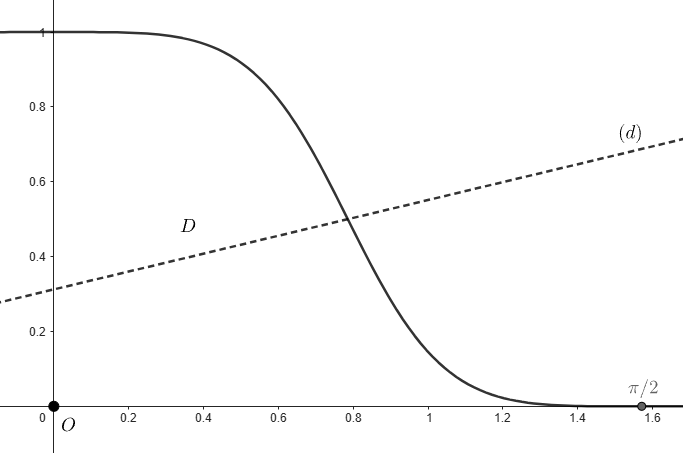
\includegraphics[width=0.5\textwidth]{Figures/05.png}
    \end{center}
    \begin{enumerate}
        \item[(a)] {Tính diện tích của $D$.}
        \item[(b)] {Cho $(d)$ là một đường thẳng đi qua hai điểm $\left(\dfrac{\pi}{4};\,\dfrac{1}{2}\right)$ và $(0;\,a)$ với $0 < a < 1$. Người ta muốn cắt $D$ dọc theo $(d)$ để thu được hai phần rời nhau có cùng diện tích (hình vẽ trong bài thể hiện một cách cắt dọc theo đường nét đứt). Coi việc cắt không làm ảnh hưởng đến diện tích của $D$. Xác định giá trị của $a$ tương ứng với một cách cắt thỏa mãn yêu cầu.} 
    \end{enumerate}
\end{tcolorbox}

\textbf{Lời giải. }

\begin{enumerate}
    \item[(a)] {Đặt $f(x) = \dfrac{(\cos x)^4}{(\sin x)^4 + (\cos x)^4}$. Phần diện tích của $D$ cần tính chính là diện tích phần không gian được giới hạn bởi các đường $y = f(x)$, trục hoành, $x = 0$ và $x = \dfrac{\pi}{2}$ nên sẽ bằng 
    $$I = \int\displaylimits_{0}^{\pi/2}\left|\dfrac{(\cos x)^4}{(\sin x)^4 + (\cos x)^4}\right|\mathrm{d}x = \int\displaylimits_{0}^{\pi/2}\dfrac{(\cos x)^4}{(\sin x)^4 + (\cos x)^4}\mathrm{d}x.$$
    
    Đổi biến $x = \dfrac{\pi}{2} - u$, để ý rằng $\sin\left(\dfrac{\pi}{2}-u\right) = \cos u$ và $\cos\left(\dfrac{\pi}{2}-u\right) = \sin u$, khi đó $$I = -\int\displaylimits_{\pi/2}^{0}\dfrac{\left(\cos \left(\dfrac{\pi}{2}-u\right)\right)^4}{\left(\sin \left(\dfrac{\pi}{2}-u\right)\right)^4 + \left(\cos \left(\dfrac{\pi}{2}-u\right)\right)^4}\mathrm{d}u = \int\displaylimits_{0}^{\pi/2}\dfrac{(\sin u)^4}{(\sin u)^4 + (\cos u)^4}\mathrm{d}u.$$
    
    Suy ra $$2I = \int\displaylimits_{0}^{\pi/2}\dfrac{(\sin x)^4}{(\sin x)^4 + (\cos x)^4}\mathrm{d}x + \int\displaylimits_{0}^{\pi/2}\dfrac{(\cos x)^4}{(\sin x)^4 + (\cos x)^4}\mathrm{d}x = \int\displaylimits_{0}^{\pi/2}\mathrm{d}x = \dfrac{\pi}{2}.$$
    
    Như vậy phần diện tích của $D$ cần tính bằng $\dfrac{\pi}{4}$.}
    \item[(b)] {Gọi $A(0;\,a)$ và $B\left(\dfrac{\pi}{4};\,\dfrac{1}{2}\right)$ lần lượt là giao điểm của đường thẳng $(d)$ với trục tung và đồ thị hàm số $y = f(x)$ như hình vẽ bên dưới.
    
    \begin{center}
        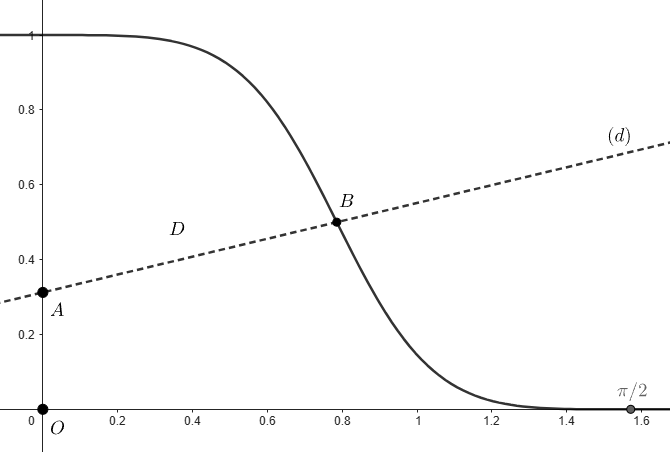
\includegraphics[width=0.5\textwidth]{Figures/06.png}
    \end{center}
    
    Vì $(d)$ đi qua $A,\,B$ nên bằng tính toán ta có được phương trình đường thẳng $(d)$ là $$y = \dfrac{2-4a}{\pi}x + a.$$
    
    Đường thẳng $(d)$ cắt $D$ thành hai phần, trong đó diện tích của phần phía trên là phần diện tích được giới hạn bởi các đường $y = f(x),\,y = \dfrac{2-4a}{\pi}x + a,\,x = 0,\,x = \dfrac{\pi}{4}$ nên bằng $$J = \int\displaylimits_{0}^{\pi/4}\left(\dfrac{(\cos x)^4}{(\sin x)^4 + (\cos x)^4} - \dfrac{2-4a}{\pi}x - a\right)\mathrm{d}x = J_1 - J_2,$$ trong đó $J_1 = \displaystyle\int\displaylimits_{0}^{\pi/4}\dfrac{(\cos x)^4}{(\sin x)^4 + (\cos x)^4}\mathrm{d}x$ và $J_2 = \displaystyle\int\displaylimits_{0}^{\pi/4}\left(\dfrac{2-4a}{\pi}x + a\right)\mathrm{d}x$.
    
    Ta có $$J_2 = \left.\left(\dfrac{1-2a}{\pi}x^2 + ax\right)\right|^{\pi/4}_{0} = \dfrac{1 - 2a}{\pi}\cdot \dfrac{\pi^2}{16} + a\cdot \dfrac{\pi}{4} = \dfrac{(1+2a)\pi}{16}.$$
    
    Với $0 \leq x \leq \dfrac{\pi}{4}$ thì $\cos x > 0$ nên ta có $J_1 = \displaystyle\int\displaylimits_{0}^{\pi/4}\dfrac{1}{(\tan x)^4 + 1}\mathrm{d}x$. Đặt $t = \tan x$ thì $\mathrm{d}t = \dfrac{1}{\cos^2 x}\mathrm{d}x = \left(\tan^2 x + 1\right)\mathrm{d}x = (t^2 + 1)\mathrm{d}x$. Khi đó 
    \begin{align*}
        J_1 &= \displaystyle\int\displaylimits_{0}^{1}\dfrac{\mathrm{d}t}{(t^2 + 1)(t^4 + 1)} = \dfrac{1}{2}\displaystyle\int\displaylimits_{0}^{1}\left(\dfrac{1}{t^2 + 1} - \dfrac{t^2 - 1}{t^4 + 1}\right)\mathrm{d}t \\
        &= \dfrac{1}{2}\int\displaylimits_{0}^{1}\dfrac{\mathrm{d}t}{t^2 + 1} + \dfrac{1}{4}\int\displaylimits_{0}^{1}\dfrac{\sqrt{2}t + 1}{t^2 + \sqrt{2}t + 1}\mathrm{d}t - \dfrac{1}{4}\int\displaylimits_{0}^{1}\dfrac{\sqrt{2}t - 1}{t^2 - \sqrt{2}t + 1}\mathrm{d}t.
    \end{align*}

    Ta có $\displaystyle\int\displaylimits_{0}^{1}\dfrac{\mathrm{d}t}{t^2 + 1} = \displaystyle\int\displaylimits_{0}^{\pi/4}\dfrac{\mathrm{d}(\tan u)}{\tan^2u + 1} = \displaystyle\int\displaylimits_{0}^{\pi/4}\dfrac{1/\cos^2u}{1/\cos^2u}\mathrm{d}u = \displaystyle\int\displaylimits_{0}^{\pi/4}\mathrm{d}u = \dfrac{\pi}{4}$.

    Tiếp theo ta lại có $\displaystyle\int\displaylimits_{0}^{1}\dfrac{\sqrt{2}t + 1}{t^2 + \sqrt{2}t + 1}\mathrm{d}t = \displaystyle\int\displaylimits_{0}^{1}\dfrac{\sqrt{2}t + 1}{\left(t + \dfrac{\sqrt{2}}{2}\right)^2 + \dfrac{1}{2}}\mathrm{d}t = \displaystyle\int\displaylimits_{\sqrt{2}/2}^{(2+\sqrt{2})/2}\dfrac{\sqrt{2}u}{u^2 + \dfrac{1}{2}}\mathrm{d}u = \dfrac{1}{\sqrt{2}}\displaystyle\int\displaylimits_{\sqrt{2}/2}^{(2+\sqrt{2})/2}\dfrac{\mathrm{d}\left(u^2 + \dfrac{1}{2}\right)}{u^2 + \dfrac{1}{2}} = \dfrac{1}{\sqrt{2}}\cdot \left.\ln \left(u^2 + \dfrac{1}{2}\right)\right|_{\sqrt{2}/2}^{(2+\sqrt{2})/2} = \dfrac{\ln (2 + \sqrt{2})}{\sqrt{2}}$.

    Và cuối cùng ta có $\displaystyle\int\displaylimits_{0}^{1}\dfrac{\sqrt{2}t - 1}{t^2 - \sqrt{2}t + 1}\mathrm{d}t = \displaystyle\int\displaylimits_{0}^{1}\dfrac{\sqrt{2}t - 1}{\left(t - \dfrac{\sqrt{2}}{2}\right)^2 + \dfrac{1}{2}}\mathrm{d}t = \displaystyle\int\displaylimits_{-\sqrt{2}/2}^{(2-\sqrt{2})/2}\dfrac{\sqrt{2}u}{u^2 + \dfrac{1}{2}}\mathrm{d}u = \dfrac{1}{\sqrt{2}}\displaystyle\int\displaylimits_{-\sqrt{2}/2}^{(2-\sqrt{2})/2}\dfrac{\mathrm{d}\left(u^2 + \dfrac{1}{2}\right)}{u^2 + \dfrac{1}{2}} = \dfrac{1}{\sqrt{2}}\cdot \left.\ln \left(u^2 + \dfrac{1}{2}\right)\right|_{-\sqrt{2}/2}^{(2-\sqrt{2})/2} = \dfrac{\ln (2 - \sqrt{2})}{\sqrt{2}}$.

    Từ đó suy ra $$J = \dfrac{\pi}{8} + \dfrac{\ln(3 + 2\sqrt{2})}{4\sqrt{2}} - \dfrac{(1+2a)\pi}{16}.$$

    Theo đề bài thì diện tích hai phần bị cắt ra từ $D$ là bằng nhau nên $J = \dfrac{\pi}{8}$, do đó $$\dfrac{\pi}{8} + \dfrac{\ln(3 + 2\sqrt{2})}{4\sqrt{2}} - \dfrac{(1+2a)\pi}{16} = \dfrac{\pi}{8} \iff a = \dfrac{\sqrt{2}\ln(3+2\sqrt{2})}{\pi} - \dfrac{1}{2}.$$

    Như vậy $a = \dfrac{\sqrt{2}\ln(3+2\sqrt{2})}{\pi} - \dfrac{1}{2}$ là giá trị $a$ cần tìm thỏa mãn yêu cầu đề bài.}
\end{enumerate}

\textbf{Nhận xét. }Bài toán là một bài ứng dụng của tích phân trong tính diện tích hình phẳng. Câu (a) là một bài toán tích phân lượng giác sử dụng phương pháp đổi biến khá quen thuộc. Lời giải được đề xuất ở đây cho câu (b) có phần hơi phức tạp hơn so với lời giải trong đáp án; tuy nhiên lời giải này sử dụng phân tách phân thức hữu tỷ và đổi biến, mà không thực hiện biến đổi lượng giác biểu thức dưới tích phân của $J_1$. Hướng giải này yêu cầu nhiều biến đổi đòi hỏi tính tỉ mỉ và cẩn thận cao, đây cũng chính là hướng giải của tác giả khi làm bài thi tại kỳ thi năm 2024; tuy nhiên khi đó vì áp lực thời gian nên tác giả chưa thể đi đến được đáp số cuối cùng.

\begin{tcolorbox}[title=\textbf{Bài toán A.4.},breakable]
    Gọi $\mathcal{F}$ là lớp tất cả các hàm $f:\,\mathbb{R}\to \mathbb{R}$ khả vi cấp hai trên $\mathbb{R}$ và có $$|f''(x)| \leq 1 \text{ với mọi }x.$$

    Hàm $f$ được gọi là có tính chất \textbf{SAT} nếu $f \in \mathcal{F}$ và $$(f'(x))^2 \leq 2024|f(x)|\text{ với mọi }x.$$

    \begin{enumerate}
        \item[(a)] {Chứng minh rằng nếu $f$ là một hàm số thuộc lớp $\mathcal{F}$ và $f(x) \geq 0$ với mọi $x \in \mathbb{R}$ thì $f$ có tính chất \textbf{SAT}.}
        \item[(b)] {Tìm một hàm số $f$ thuộc lớp $\mathcal{F}$ nhưng $f$ không có tính chất \textbf{SAT}.}  
    \end{enumerate}
\end{tcolorbox}

\textbf{Lời giải. }

\begin{enumerate}
    \item[(b)] {
        Xét hàm số $f(x) = \dfrac{x}{2x^2 + 2}$ xác định trên $\mathbb{R}$ và có $f'(x) = \dfrac{1-x^2}{2(x^2 + 1)^2},\,f''(x) = \dfrac{x(x^2 - 3)}{(x^2+1)^3}$ và $f'''(x) = \dfrac{-3(x^4-6x^2+1)}{(x^2+1)^4}$.

        \begin{center}
            \begin{tikzpicture}[yscale=.8,xscale=1.5,thick]
            \definecolor{belize}{RGB}{41, 128, 185}
            \definecolor{midblue}{RGB}{44, 62, 80}
            % \definecolor{sun}{RGB}{241, 196, 15}
            \begin{scope}[shift={(-.5,.5)}]
            % \fill[sun!20] (0,0) rectangle +(8,-6) ;
            \draw[midblue]
            (0,0) rectangle +(9.5,-9) 
            (0,-1)--+(0:9.5)
            (0,-2)--+(0:9.5)
            (1,0)--+(-90:9)
            ;
            \end{scope}
            \path
            (0,0) node{$x$} % <<< Dòng 1
            ++(0:1) node{$-\infty$}
            ++(0:1.5) node(A){$-1-\sqrt{2}$}
            ++(0:1.5) node{$1-\sqrt{2}$}
            ++(0:1.5) node{$-1+\sqrt{2}$}
            ++(0:1.5) node{$1+\sqrt{2}$}
            ++(0:1.5) node{$+\infty$}
            
            (0,-1)   node{$f'''(x)$}  % <<< Dòng 2
            ++(0:1.5) node {$-$}
            ++(0:1.1) node (D) {$0$}
            ++(0:0.75) node {$+$}
            ++(0:0.75) node (F) {$0$}
            ++(0:0.75) node {$-$}
            ++(0:0.75) node {$0$}
            ++(0:0.75) node {$+$}
            ++(0:0.75) node {$0$}
            ++(0:0.75) node {$-$}
            ++(0:1)++(0:1) node (G) {}
            
            (0,-2)   node{$f''(x)$}  % <<< Dòng 3
            ++(0:1)++(-90:2) node (L) {$0$}
            ++(0:1.5)++(-90:2) node (M) {$\dfrac{2\sqrt{2}-3}{8}$}
            ++(0:1)++(90:1) coordinate (N)
            ++(0:0.5)++(90:2.5) node (O) {$\dfrac{2\sqrt{2}+3}{8}$}
            ++(0:1.5)++(-90:5) node (P) {$\dfrac{-2\sqrt{2}-3}{8}$}
            ++(0:1.5)++(90:4) node (Q) {$\dfrac{-2\sqrt{2}+3}{8}$}
            ++(0:1.5)++(-90:0.5) node (R) {$0$};
    
            % (6.25, 0) node (X) {\textcolor{red}{$x_0$}}
            % (6.25, -2.75) node (Y) {\textcolor{red}{$\bullet$}}
            % (6.25, -3.25) node {\textcolor{red}{$y_0$}}; 
            
            % \draw[-stealth,blue,dashed,shorten <=5] (X)--(Y);
            \draw[-stealth] (L)--(M);
            \draw[-stealth] (M)--(O);
            \draw[-stealth] (O)--(P);
            \draw[-stealth] (P)--(Q);
            \draw[-stealth] (Q)--(R);
            \end{tikzpicture}
        \end{center}

        Dựa vào bảng biến thiên, ta thấy $-1 < f''(x) < 1$ hay $|f''(x)| < 1$ với mọi $x \in \mathbb{R}$ nên $f\in \mathcal{F}$.

        Ta sẽ chứng minh rằng hàm $f$ nói trên không có tính chất \textbf{SAT}, hay tồn tại $x_0$ để $$\left(f'(x_0)\right)^2 > 2024|f(x_0)| \iff \dfrac{(1-x_0^2)^2}{4(x_0^2+1)^4} > \dfrac{2024|x_0|}{2x_0^2+2} \iff \dfrac{(1-x_0^2)^2}{|x_0|(x_0^2+1)^3}>4048.$$

        Thật vậy, vì $\lim\limits_{x \to 0} \dfrac{(1-x^2)^2}{(x^2+1)^3} = 1,\,\lim\limits_{x \to 0} |x| = 0$ nên ta có $\lim\limits_{x \to 0} \dfrac{(1-x^2)^2}{|x|(x^2+1)^3} = +\infty$. Do đó chỉ cần chọn $x_0$ đủ nhỏ thì ta có ngay $\dfrac{(1-x_0^2)^2}{|x_0|(x_0^2+1)^3}>4048$. Như vậy hàm $f$ nói trên thuộc $\mathcal{F}$ nhưng không có tính chất \textbf{SAT}.
    }
\end{enumerate}

\textbf{Nhận xét. }Câu (b) của bài toán nếu xét hàm $f(x) = \sin x$ thì việc giải quyết sẽ đơn giản hơn nhiều, tuy nhiên tác giả muốn thử thách hơn bằng việc tìm một hàm khác hàm lượng giác. Vì hàm cần tìm phải thỏa $|f''(x)| \leq 1$ nên nếu chọn hàm thỏa $|f(x)| \leq 1$ thì khả năng điều kiện trên cũng thỏa, nên sẽ thử chọn hàm $f$ có dạng $\dfrac{1}{g(x)}$. Lúc này thử chọn $g(x)$ là một đại lượng điều hòa $x + \dfrac{1}{x}$, tức khi đó $f(x) = \dfrac{1}{x + \dfrac{1}{x}} = \dfrac{x}{x^2 + 1}$ thì may mắn $|f''(x)| \leq 2$ và tồn tại $x_0$ để $\left(f'(x_0)\right)^2 > 2024|f(x_0)|$. Lúc này chỉ việc nhân thêm $\dfrac{1}{2}$ vào $f(x)$ để $|f''(x)| \leq 1$ là xong.

Ngoài ra, ở câu (b) ta cũng có thể chọn hàm đa thức thỏa mãn $f''(x) = 1$ với mọi $x$, tức $f'(x) = x + c_1$ và $f(x) = \dfrac{x^2}{2} + c_1x + c_2$. Khi đó cần chọn $c_1,\,c_2$ để tồn tại $x_0$ thỏa mãn $(f'(x_0))^2 > 2024|f(x_0)| \iff x_0^2 + 2c_1x_0 + c_1^2 > 2024\left|\dfrac{x_0^2}{2} + c_1x_0 + c_2\right|$. Giả sử chọn $x_0 = 0$ thì cần chọn $c_1,\,c_2$ thỏa mãn $c_1^2 > 2024|c_2|$. Đến đây thấy ngay một cặp $(c_1,\,c_2) = (1,\,0)$ thỏa mãn. Điều đó có nghĩa là $f(x) = \dfrac{x^2}{2} + x$ cũng là một ví dụ hàm $f$ trong câu (b). Việc tìm ra hàm số này là khả thi hơn trong điều kiện phòng thi, so với hàm số trong lời giải trên.

\begin{tcolorbox}[title=\textbf{Bài toán A.5.},breakable]
    Cho $f:\,[0;\,+\infty) \to \mathbb{R}$ là một hàm số khả vi sao cho giới hạn $$\lim\limits_{x \to +\infty} \int\displaylimits_{0}^{x}f^2(t)\mathrm{d}t$$ tồn tại và hữu hạn.

    \begin{enumerate}
        \item[(a)] {Cho một ví dụ về hàm số $f$ thỏa mãn tất cả các yêu cầu trên.}
        \item[(b)] {Chứng minh rằng nếu $f'$ bị chặn trên $[0;\,+\infty)$ thì $$\lim\limits_{x \to +\infty}f(x) = 0.$$}  
        \item[(c)] {Khẳng định trong ý (b) có còn đúng không nếu ta không giả thiết $f'$ bị chặn trên $[0;\,+\infty)$ (nếu câu trả lời là ``có'', hãy chứng minh; nếu câu trả lời là ``không'', hãy chỉ ra ví dụ về một hàm $f$)?}
    \end{enumerate}
\end{tcolorbox}

\textbf{Lời giải. }

\begin{enumerate}
    \item[(a)] {Xét hàm số $f(x) = 2024^{-x}$ khả vi trên $\mathbb{R}$ và $$\lim\limits_{x \to +\infty} \int\displaylimits_{0}^{x}f^2(t)\mathrm{d}t = \lim\limits_{x \to +\infty} \int\displaylimits_{0}^{x}2024^{-2t}\mathrm{d}t = \lim\limits_{x \to +\infty} \dfrac{1}{(-2) \cdot \ln 2024} \left(2024^{-2x} - 1\right) = \dfrac{1}{2 \cdot \ln 2024}.$$}
\end{enumerate}

\textbf{Nhận xét. }Ở câu (a), mục tiêu ta cần phải chọn hàm $f$ thỏa mãn $\lim\limits_{x \to +\infty}f(x)$ hữu hạn $\left(\text{thì khi đó khả năng $\displaystyle\lim\limits_{x \to +\infty} \int\displaylimits_{0}^{x}f^2(t)\mathrm{d}t$ tồn tại và hữu hạn}\right)$, đồng thời khi bình phương lẫn lấy nguyên hàm thì không làm mất tính chất của hàm đó và việc lấy nguyên hàm được thực hiện dễ dàng. Như vậy thấy ngay hàm mũ $f(x) = a^{-x}$ là đáp ứng được những yêu cầu này.